\documentclass[12pt]{article}

%% Created with wxMaxima 12.04.0

\usepackage[english]{babel}
\usepackage[utf8x]{inputenc}
\usepackage{amsmath}
\usepackage{graphicx}
\usepackage{ulem}
\usepackage{placeins}
\usepackage[colorinlistoftodos]{todonotes}
\usepackage{listings}
\usepackage{glossaries}
\usepackage[
top    = 2.75cm,
bottom = 2.00cm,
left   = 2.50cm,
right  = 2.00cm]{geometry}
\setcounter{secnumdepth}{4}
\setlength{\parskip}{\medskipamount}
\setlength{\parindent}{0pt}

\definecolor{labelcolor}{RGB}{100,0,0}

\begin{document}

\pagebreak{}
{\Huge {\sc Statistik und Wahrscheinlichkeitsrechnung
S06  -  Siegel Hannah  -  5AHITT}}
\setcounter{section}{0}
\setcounter{subsection}{0}
\setcounter{figure}{0}



\subsection{Bloecke}



\noindent
%%%%%%%%%%%%%%%
%%% INPUT:
\begin{minipage}[t]{8ex}{\color{red}\bf
\begin{verbatim}
(%i1) 
\end{verbatim}}
\end{minipage}
\begin{minipage}[t]{\textwidth}{\color{blue}
\begin{verbatim}
kill(all);
load(descriptive)$
load(draw)$
\end{verbatim}}
\end{minipage}
%%% OUTPUT:
\begin{math}\displaystyle
\parbox{8ex}{\color{labelcolor}(\%o0) }
done
\end{math}
%%%%%%%%%%%%%%%

Der Block  rand\_col returnt eine schoene farbe nach zufallsprinzip.
    intnum ... 1 = pink - ton
               2 = blau - ton
               3 = grau - ton

\noindent
%%%%%%%%%%%%%%%
%%% INPUT:
\begin{minipage}[t]{8ex}{\color{red}\bf
\begin{verbatim}
(%i3) 
\end{verbatim}}
\end{minipage}
\begin{minipage}[t]{\textwidth}{\color{blue}
\begin{verbatim}
rand_col(intnum):=block(
    colors[1]:[magenta,dark-magenta, violet, dark-violet, plum, purple, light-pink, dark-pink,salmon],
    colors[2]:[cyan,dark-blue,skyblue,navy,light-blue,blue,dark-cyan],
    colors[3]:[gray10,gray20,gray30,gray40,gray50,gray60,gray70,gray80,gray90],
    colors[intnum][random(length(colors[intnum])-1)+1]
)$
\end{verbatim}}
\end{minipage}

Der Block  prepare\_list nimmt die basis liste der werte 
    (urliste in dem Format [[ Fehler1, FehlerBezeichnung1],[ Fehler2, FehlerBezeichnung2],..] ) 
    und formt sie auf [[1,2,3...],[FehlerBezeichnung1 ,FehlerBezeichnung5, FehlerBezeichnung3,...],[ Fehler1,  Fehler5,  Fehler3, ...]] um.
Weiters wird die Liste nach der groesse der Fehler sortiert. 
Prinzipiell wird dieser Block eigenstaendig von draw\_pareto und draw\_piechart aufgerufen.

\noindent
%%%%%%%%%%%%%%%
%%% INPUT:
\begin{minipage}[t]{8ex}{\color{red}\bf
\begin{verbatim}
(%i4) 
\end{verbatim}}
\end{minipage}
\begin{minipage}[t]{\textwidth}{\color{blue}
\begin{verbatim}
prepare_list(list_angabe):=block(
    list_angabe:sort(list_angabe,ordergreatp),
    angabe_beschriftung:[],
 angabe_wert:[],
    angabe_inkr:[],
    for i:1 while i<= length(list_angabe) do [
        angabe_beschriftung: append(angabe_beschriftung,[list_angabe[i][2]]),
        angabe_wert: append(angabe_wert,[list_angabe[i][1]]),
        angabe_inkr: append(angabe_inkr,[i])
    ],
    list_angabe:[angabe_inkr,angabe_beschriftung,angabe_wert]
)$
\end{verbatim}}
\end{minipage}

Der Block  draw\_pareto nimmt die basis liste der werte 
    (urliste in dem Format [[ Fehler1, FehlerBezeichnung1],[ Fehler2, FehlerBezeichnung2],..] )
und zeichnet ein Paretto Diagramm

\noindent
%%%%%%%%%%%%%%%
%%% INPUT:
\begin{minipage}[t]{8ex}{\color{red}\bf
\begin{verbatim}
(%i5) 
\end{verbatim}}
\end{minipage}
\begin{minipage}[t]{\textwidth}{\color{blue}
\begin{verbatim}
draw_pareto(list_angabe):=block(
  list_angabe:prepare_list(list_angabe),
  wxdraw2d(
        xrange=[0,length(list_angabe[3])+1], 
        yrange=[lmin(list_angabe[3])-1,lmax(list_angabe[3])+1], 
        xaxis=true, 
        yaxis=true, 
        grid=true, 
        xtics=1, 
        ytics=5,
        points_joined = impulses,
        color=rand_col(1),
        line_width=10,
        points(list_angabe[1],list_angabe[3]),
        xlabel="Fehler", ylabel="Anzahl"
   )
)$
\end{verbatim}}
\end{minipage}

Der Block  draw\_piechart nimmt die basis liste der werte 
    (urliste in dem Format [[ Fehler1, FehlerBezeichnung1],[ Fehler2, FehlerBezeichnung2],..] )
und zeichnet ein Torten Diagramm

\noindent
%%%%%%%%%%%%%%%
%%% INPUT:
\begin{minipage}[t]{8ex}{\color{red}\bf
\begin{verbatim}
(%i6) 
\end{verbatim}}
\end{minipage}
\begin{minipage}[t]{\textwidth}{\color{blue}
\begin{verbatim}
draw_piechart(list_angabe):=block(
  list_angabe:prepare_list(list_angabe),
  list:[],
  for i:1 while i <= length(list_angabe[1]) do [
    list: append(list, makelist(list_angabe[2][i],j,1,list_angabe[3][i]))
  ],
  wxpiechart(
        list,
        proportional_axes=xy,
        xrange=[-1.03,3], 
        yrange=[-1.03,1.03],
        xtics=false,
        ytics=false,
        sector_colors = [magenta,dark-magenta, violet, dark-violet, plum, purple, light-pink, dark-pink,salmon],
        title="Fehler"
    )
)$
\end{verbatim}}
\end{minipage}

Der Block klassenbildung hat folgende eingangsparameter:
    messwerte: messwerte
    steps: Klassenbreite W
    anzahl\_klassen: anzahl der zu bildenden Klassen
Folgende ausgangsparameter:
    klassen: liste der gebildeten Klassen
    end\_list: neue liste im Format: [1,2,6,2,8,3,5,1,5,7,8,3,7,... ]

\noindent
%%%%%%%%%%%%%%%
%%% INPUT:
\begin{minipage}[t]{8ex}{\color{red}\bf
\begin{verbatim}
(%i7) 
\end{verbatim}}
\end{minipage}
\begin{minipage}[t]{\textwidth}{\color{blue}
\begin{verbatim}
klassenbildung(messwerte,steps, anzahl_klassen):=block(
  xmin: lmin(messwerte),
  xmax: lmax(messwerte),
  klassen:[[0,xmin+2*steps]],
    xmin:xmin+2*steps,
  for j:1 while j<anzahl_klassen do [
    neuer_kleinstwert:xmin+steps,
    klassen:append(klassen, [[xmin,neuer_kleinstwert]]),
    xmin:neuer_kleinstwert
  ],
  klassen[anzahl_klassen][2]:100000,  
  for n:1 while n<=length(klassen) do [
    class[n]:[]
  ],
  end_list:[],
  for i:1 while i<=length(messwerte) do [ 
    for j:1 while j<= length(klassen) do [
        if (messwerte[i] > klassen[j][1] ) then if( messwerte[i] <= klassen[j][2]) then end_list:append( end_list,[j])
    ]
  ]
)$
\end{verbatim}}
\end{minipage}

Der Block get\_labels stueckelt die Klassen in ein labels object, welches nachher dann in die Grafik eingebunden werden kann.

    klassen ... Klassen welche nach dem Aufruf des klassenbildungs-blockes verfuegbar sind
    delta\_minus ... Platz zum Zeichnen der Labels in die negative Richtung

\noindent
%%%%%%%%%%%%%%%
%%% INPUT:
\begin{minipage}[t]{8ex}{\color{red}\bf
\begin{verbatim}
(%i8) 
\end{verbatim}}
\end{minipage}
\begin{minipage}[t]{\textwidth}{\color{blue}
\begin{verbatim}
get_labels(klassen,delta_minus):=block(
  a:label(),
  int_place1:-(delta_minus*0.25),
  int_place2:-(delta_minus*0.75),
  for i:1 while i<= length(klassen) do [
        num:concat("[",klassen[i][1],",",klassen[i][2],"]"),
        if (evenp(i)=true) then a: append(a,label([num,i,int_place1])),
        if (evenp(i)=false) then a: append(a,label([num,i,int_place2]))
  ],
  label_arr:a
)$
\end{verbatim}}
\end{minipage}

--------------------------------------------- draw\_normal\_generalized -----------------------------------------
draw\_normal\_generalized
    Der draw\_normal\_generalized Block, zeichnet die normalen Grafiken der Statistik.

    Er wird von den anderen draw\_ Bloecken aufgerufen und sollte fuer den User niemals von Bedeutung sein.


draw\_normal\_generalized(ytics\_value,title\_grafik,ylabel\_grafik,balken,list\_discrete)

title\_grafik    ... Titel der Grafik
ylabel\_grafik   ... Beschriftung der y\_achse (ob Prozente oder Anzahl)
balken          ... bars() object
ytics\_value     ... Abstand der Werte auf der y-Achse (Default:5)
list\_discrete   ... die discrete liste, zum berechnen der ranges benoetigt 

\noindent
%%%%%%%%%%%%%%%
%%% INPUT:
\begin{minipage}[t]{8ex}{\color{red}\bf
\begin{verbatim}
(%i9) 
\end{verbatim}}
\end{minipage}
\begin{minipage}[t]{\textwidth}{\color{blue}
\begin{verbatim}
draw_normal_generalized(ytics_value,title_grafik,ylabel_grafik,balken,list_discrete) := block(
     wxdraw2d(
        xrange=[lmin(list_discrete[1])-1,lmax(list_discrete[1])+1], 
        yrange=[0,ceiling (lmax(list_discrete[2])+(lmax(list_discrete[2])/10))],
        xaxis=true, yaxis=true,
        grid=true,
        xtics=1, 
        ytics=ytics_value,
        fill_color=rand_col(1),
        balken,
        title=title_grafik,
        xlabel="Messwert", ylabel=ylabel_grafik
    )
)$
\end{verbatim}}
\end{minipage}

--------------------------------------------- draw\_klassen\_generalized -----------------------------------------
draw\_klassen\_generalized
    Der draw\_klassen\_generalized Block, zeichnet die normalen Grafiken der Statistik.

    Er wird von den anderen draw\_ Bloecken aufgerufen und sollte fuer den User niemals von Bedeutung sein.
draw\_normal\_generalized(xdimension,ydimension,ylabel\_grafik,title\_grafik,list\_discrete,labels\_list,balken,ytics\_value,delta\_minus)
title\_grafik    ... Titel der Grafik
ylabel\_grafik   ... Beschriftung der y\_achse (ob Prozente oder Anzahl)
balken          ... bars() object
ytics\_value     ... Abstand der Werte auf der y-Achse
list\_discrete   ... die discrete liste, zum berechnen der ranges benoetigt 
xdimension      ... Groesse der Zeichnung nach x (Default:500)
ydimension      ... Groesse der Zeichnung nach y (Default:300)
labels\_list     ... labels() object
delta\_minus     ... POSITIVER Wert, range fuer das anzeigen der Labels (sollte meist zwischen ca 5 und 20 liegen)

\noindent
%%%%%%%%%%%%%%%
%%% INPUT:
\begin{minipage}[t]{8ex}{\color{red}\bf
\begin{verbatim}
(%i10) 
\end{verbatim}}
\end{minipage}
\begin{minipage}[t]{\textwidth}{\color{blue}
\begin{verbatim}
draw_klassen_generalized(xdimension,ydimension,ylabel_grafik,title_grafik,list_discrete,labels_list,balken,ytics_value,delta_minus) := block(
     wxdraw2d(
        xrange=[lmin(list_discrete[1])-1,lmax(list_discrete[1])+1], 
        yrange=[-delta_minus,ceiling (lmax(list_discrete[2])+(lmax(list_discrete[2])/10))],
        xaxis=false, 
        yaxis=false, 
        grid=true,
        xtics=false, 
        ytics=ytics_value,
        color=black,
        line_type=solid,
        font_size=11, 
        font="Arial",
        dimensions = [xdimension, ydimension],
        labels_list,
        font_size=10,
        fill_color=rand_col(1),
        balken,
        xlabel="Klassen", 
        ylabel=ylabel_grafik,
        title=title_grafik
    )
)$
\end{verbatim}}
\end{minipage}

--------------------------------------------- draw\_\verb|<|TYPE\verb|>|\_klassen -----------------------------------------

draw\_TYPE\_klassen
    Jeder draw\_TYPE\_klassen Block, macht die Klasseneinteilung sowie das Zeichnen mit den Labels automatisch.
    Die Bloecke dienen nur zur abstraktion sowie hilfe fuer den User, um die verwendung des tatsaechlichens draw-Blocks zu vermeiden


draw\_TYPE\_klassen(messwerte,steps,anzahl\_klasse,ytics,delta\_minus,xdimension,ydimension)

messwerte       ... Eine Liste der messwerte im Format [Messwert1, Messwert2, ...]
steps           ... Die Klassenbreite W
anzahl\_klassen  ... Anzahl der Klassen
ytics           ... Abstand der Werte auf der y-Achse
delta\_minus     ... POSITIVER Wert, range fuer das anzeigen der Labels (sollte meist zwischen ca 5 und 20 liegen)
xdimension      ... Groesse der Zeichnung nach x (Default:500)
ydimension      ... Groesse der Zeichnung nach y (Default:300)

\noindent
%%%%%%%%%%%%%%%
%%% INPUT:
\begin{minipage}[t]{8ex}{\color{red}\bf
\begin{verbatim}
(%i11) 
\end{verbatim}}
\end{minipage}
\begin{minipage}[t]{\textwidth}{\color{blue}
\begin{verbatim}
draw_KUM_ABS_HFG_klassen(messwerte,steps,anzahl_klassen,ytics_value,delta_minus,groesse1,groesse2):=block(
  klassenbildung(messwerte,steps, anzahl_klassen),
  if (delta_minus = 0) then delta_minus:15,
  get_labels(klassen,delta_minus),
  draw_KUM_ABS_HFG(end_list,ytics_value,false,label_arr,delta_minus,groesse1,groesse2)
)$
\end{verbatim}}
\end{minipage}


\noindent
%%%%%%%%%%%%%%%
%%% INPUT:
\begin{minipage}[t]{8ex}{\color{red}\bf
\begin{verbatim}
(%i12) 
\end{verbatim}}
\end{minipage}
\begin{minipage}[t]{\textwidth}{\color{blue}
\begin{verbatim}
draw_RELATIVE_HFG_klassen(messwerte,steps,anzahl_klassen,ytics_value,delta_minus,groesse1,groesse2):=block(
  klassenbildung(messwerte,steps, anzahl_klassen),
  if (delta_minus = 0) then delta_minus:5,
  get_labels(klassen,delta_minus),
  draw_RELATIVE_HFG(end_list,ytics_value,false,label_arr,delta_minus,groesse1,groesse2)
)$
\end{verbatim}}
\end{minipage}


\noindent
%%%%%%%%%%%%%%%
%%% INPUT:
\begin{minipage}[t]{8ex}{\color{red}\bf
\begin{verbatim}
(%i13) 
\end{verbatim}}
\end{minipage}
\begin{minipage}[t]{\textwidth}{\color{blue}
\begin{verbatim}
draw_KUM_REL_HFG_klassen(messwerte,steps,anzahl_klassen,ytics_value,delta_minus,groesse1,groesse2):=block(
  klassenbildung(messwerte,steps, anzahl_klassen),
  if (delta_minus = 0) then delta_minus:20,
  get_labels(klassen,delta_minus),
  draw_KUM_REL_HFG(end_list,ytics_value,false,label_arr,delta_minus,groesse1,groesse2)
)$
\end{verbatim}}
\end{minipage}


\noindent
%%%%%%%%%%%%%%%
%%% INPUT:
\begin{minipage}[t]{8ex}{\color{red}\bf
\begin{verbatim}
(%i14) 
\end{verbatim}}
\end{minipage}
\begin{minipage}[t]{\textwidth}{\color{blue}
\begin{verbatim}
draw_ABSOLUTE_HFG_klassen(messwerte,steps,anzahl_klassen,ytics_value,delta_minus,groesse1,groesse2):=block(
  klassenbildung(messwerte,steps, anzahl_klassen),
  if (delta_minus = 0) then delta_minus:5,
  get_labels(klassen,delta_minus),
  draw_ABSOLUTE_HFG(end_list,ytics_value,false,label_arr,delta_minus,groesse1,groesse2)
)$
\end{verbatim}}
\end{minipage}

--------------------------------------------- draw\_\verb|<|TYPE\verb|>|\_normal -----------------------------------------

draw\_TYPE\_normal
    Jeder draw\_TYPE\_normal Block, ruft den komplitzierten draw Block auf, und uebergibt ihm die richtigen Parameter


draw\_TYPE\_normal(list\_angabe,ytics\_value)

list\_angabe       ... Eine Liste der messwerte im Format [Messwert1, Messwert2, ...]
ytics\_value     ... Abstand der Werte auf der y-Achse (Default:5)

\noindent
%%%%%%%%%%%%%%%
%%% INPUT:
\begin{minipage}[t]{8ex}{\color{red}\bf
\begin{verbatim}
(%i15) 
\end{verbatim}}
\end{minipage}
\begin{minipage}[t]{\textwidth}{\color{blue}
\begin{verbatim}
draw_KUM_ABS_HFG_normal(list_angabe,ytics_value):=block(
  draw_KUM_ABS_HFG(list_angabe,ytics_value,true,0,0,0,0)
)$
\end{verbatim}}
\end{minipage}


\noindent
%%%%%%%%%%%%%%%
%%% INPUT:
\begin{minipage}[t]{8ex}{\color{red}\bf
\begin{verbatim}
(%i16) 
\end{verbatim}}
\end{minipage}
\begin{minipage}[t]{\textwidth}{\color{blue}
\begin{verbatim}
draw_KUM_REL_HFG_normal(list_angabe,ytics_value):=block(
  draw_KUM_REL_HFG(list_angabe,ytics_value,true,0,0,0,0)
)$
\end{verbatim}}
\end{minipage}


\noindent
%%%%%%%%%%%%%%%
%%% INPUT:
\begin{minipage}[t]{8ex}{\color{red}\bf
\begin{verbatim}
(%i17) 
\end{verbatim}}
\end{minipage}
\begin{minipage}[t]{\textwidth}{\color{blue}
\begin{verbatim}
draw_ABSOLUTE_HFG_normal(list_angabe,ytics_value):=block(
  draw_ABSOLUTE_HFG(list_angabe,ytics_value,true,0,0,0,0)
)$
\end{verbatim}}
\end{minipage}


\noindent
%%%%%%%%%%%%%%%
%%% INPUT:
\begin{minipage}[t]{8ex}{\color{red}\bf
\begin{verbatim}
(%i18) 
\end{verbatim}}
\end{minipage}
\begin{minipage}[t]{\textwidth}{\color{blue}
\begin{verbatim}
draw_RELATIVE_HFG_normal(list_angabe,ytics_value):=block(
  draw_RELATIVE_HFG(list_angabe,ytics_value,true,0,0,0,0)
)$
\end{verbatim}}
\end{minipage}

--------------------------------------------- draw\_\verb|<|TYPE\verb|>| ---------------------------------------------

draw\_TYPE
    Jeder draw\_TYPE Block, berechnet und zeichnet die jeweiligen Darstellungen. 
    Jeder draw\_TYPE Block kann sowohl die normale als auch die komplizierte Klassen darstellung zeichnen.

draw\_TYPE\_klassen(messwerte,ytics,normal\_bool,labels,delta\_minus,xdimension,ydimension)

messwerte       ... Eine Liste der messwerte im Format [Messwert1, Messwert2, ...]
normal\_bool     ... true = normal ; false = mit labels und allem dazugehoerigen berechnungen
labels\_list     ... Liste der Labels welche nach dem Aufruf get\_labels vorhanden ist.
ytics           ... Abstand der Werte auf der y-Achse
delta\_minus     ... POSITIVER Wert, range fuer das anzeigen der Labels (sollte meistens zwischen ca 5 und 20 liegen)
xdimension      ... Groesse der Zeichnung nach x (Default:500)
ydimension      ... Groesse der Zeichnung nach y (Default:300)

\noindent
%%%%%%%%%%%%%%%
%%% INPUT:
\begin{minipage}[t]{8ex}{\color{red}\bf
\begin{verbatim}
(%i19) 
\end{verbatim}}
\end{minipage}
\begin{minipage}[t]{\textwidth}{\color{blue}
\begin{verbatim}
draw_ABSOLUTE_HFG(list_angabe,ytics_value,normal_bool,labels_list,delta_minus,xdimension,ydimension):=block(
    list_discrete:discrete_freq(list_angabe),
    r:bars(),
    if (xdimension = 0) then xdimension:500,
    if (ydimension = 0) then ydimension:300,
    if (ytics_value = 0) then ytics_value:5,
    for i:1 while i<=length(list_discrete[1]) do [
        r: append(r, bars([list_discrete[1][i],list_discrete[2][i],0.5]))
    ],
    if (normal_bool=true) then
        draw_normal_generalized(ytics_value,"Absolute Haeufigkeit","Anzahl",r,list_discrete)
    else
    if (normal_bool=false) then
        draw_klassen_generalized(xdimension,ydimension,"Anzahl","Absolute Haeufigkeit",list_discrete,labels_list,r,ytics_value,delta_minus)
)$
\end{verbatim}}
\end{minipage}


\noindent
%%%%%%%%%%%%%%%
%%% INPUT:
\begin{minipage}[t]{8ex}{\color{red}\bf
\begin{verbatim}
(%i20) 
\end{verbatim}}
\end{minipage}
\begin{minipage}[t]{\textwidth}{\color{blue}
\begin{verbatim}
draw_KUM_ABS_HFG(list_angabe,ytics_value,normal_bool,labels_list,delta_minus,xdimension,ydimension):=block(
    list_discrete:discrete_freq(list_angabe),
    if (xdimension = 0) then xdimension:500,
    if (ydimension = 0) then ydimension:300,
    if (ytics_value = 0) then ytics_value:10,
    neu1:[],
    neu2:[],
    found:1,
    sum:0,
    neue_werte:[],
    for n:1 while n<=length(list_discrete[2]) do [
        neuer_wert: list_discrete[2][n]+sum,
        sum : sum + list_discrete[2][n],
        neue_werte:append(neue_werte,[neuer_wert])
    ],
    abs_hf:[list_discrete[1],neue_werte],
    for k:lmin(abs_hf[1]) while k<=lmax(abs_hf[1]) do [
        neu1:append(neu1,[k]),
        if ((member(k,abs_hf[1]))) then neu2:append(neu2,[abs_hf[2][found]]),
        if ((member(k,abs_hf[1]))) then found:found+1,
        if (not(member(k,abs_hf[1]))) then neu2:append(neu2,[neu2[k-lmin(abs_hf[1])]])
    ],  
    list_discrete:[neu1,neu2],
    r:bars(),
    for i:1 while i<=length(list_discrete[1]) do [
        r: append(r, bars([list_discrete[1][i],list_discrete[2][i],0.5]))
    ],
    if (normal_bool = true) then
        draw_normal_generalized(ytics_value,"Kummulative Absolute Haeufigkeit","Anzahl",r,list_discrete)
    else
    if (normal_bool = false) then
      draw_klassen_generalized(xdimension,ydimension,"Anzahl","Kummulative Absolute Haeufigkeit",list_discrete,labels_list,r,ytics_value,delta_minus)
)$
\end{verbatim}}
\end{minipage}


\noindent
%%%%%%%%%%%%%%%
%%% INPUT:
\begin{minipage}[t]{8ex}{\color{red}\bf
\begin{verbatim}
(%i21) 
\end{verbatim}}
\end{minipage}
\begin{minipage}[t]{\textwidth}{\color{blue}
\begin{verbatim}
draw_KUM_REL_HFG(list_angabe,ytics_value,normal_bool,labels_list,delta_minus,xdimension,ydimension):=block(
   list_discrete:discrete_freq(list_angabe),
    if (xdimension = 0) then xdimension:500,
    if (ydimension = 0) then ydimension:300,
    if (ytics_value = 0) then ytics_value:10,
    prozente:[],
    for n:1 while n<=length(list_discrete[2]) do [
        prozent: (100/length(list_angabe)) * list_discrete[2][n],
        prozent: round(prozent),
        prozente:append(prozente,[prozent])
    ],
    list_discrete:[list_discrete[1],prozente],
    neu1:[],
    neu2:[],
    found:1,
    sum:0,
    neue_werte:[],
    for n:1 while n<=length(list_discrete[2]) do [
        neuer_wert: list_discrete[2][n]+sum,
        sum : sum + list_discrete[2][n],
        neue_werte:append(neue_werte,[neuer_wert])
    ],
    abs_hf:[list_discrete[1],neue_werte],
    for k:lmin(abs_hf[1]) while k<=lmax(abs_hf[1]) do [
        neu1:append(neu1,[k]),
        if ((member(k,abs_hf[1]))) then neu2:append(neu2,[abs_hf[2][found]]),
if ((member(k,abs_hf[1]))) then found:found+1,
        if (not(member(k,abs_hf[1]))) then neu2:append(neu2,[neu2[k-lmin(abs_hf[1])]])
  ],  
    list_discrete:[neu1,neu2],
    r:bars(),
    for i:1 while i<=length(list_discrete[1]) do [
        r: append(r, bars([list_discrete[1][i],list_discrete[2][i],0.5]))
    ],
    if (normal_bool=true) then
        draw_normal_generalized(ytics_value,"Kummulative Relative Haeufigkeit","Prozent",r,list_discrete)
    else
    if (normal_bool=false) then
        draw_klassen_generalized(xdimension,ydimension,"Prozent","Kummulative Relative Haeufigkeit",list_discrete,labels_list,r,ytics_value,delta_minus)
)$
\end{verbatim}}
\end{minipage}


\noindent
%%%%%%%%%%%%%%%
%%% INPUT:
\begin{minipage}[t]{8ex}{\color{red}\bf
\begin{verbatim}
(%i22) 
\end{verbatim}}
\end{minipage}
\begin{minipage}[t]{\textwidth}{\color{blue}
\begin{verbatim}
draw_RELATIVE_HFG(list_angabe,ytics_value,normal_bool,labels_list,delta_minus,xdimension,ydimension):=block(
    prozente:[],
    if (xdimension = 0) then xdimension:500,
    if (ydimension = 0) then ydimension:300,
    if (ytics_value = 0) then ytics_value:5,
    list_discrete:discrete_freq(list_angabe),
    for n:1 while n<=length(list_discrete[2]) do [
        prozent: (100/length(list_angabe)) * list_discrete[2][n],
        prozent: float(prozent),
        prozent: round(prozent),
        prozente:append(prozente,[prozent])
    ],
    list_discrete:[list_discrete[1],prozente],
    r:bars(),
    for i:1 while i<=length(list_discrete[1]) do [
        r: append(r, bars([list_discrete[1][i],list_discrete[2][i],0.5]))
    ],
    if (normal_bool = true) then
        draw_normal_generalized(ytics_value,"Relative Haeufigkeit","Prozent",r,list_discrete)    
    else
    if (normal_bool = false) then
        draw_klassen_generalized(xdimension,ydimension,"Prozent","Relative Haeufigkeit",list_discrete,labels_list,r,ytics_value,delta_minus)
)$
\end{verbatim}}
\end{minipage}

Block fuer das Zeichnen von Punkten als Punkte:
    list\_angabe ... angabe der Punkte

\noindent
%%%%%%%%%%%%%%%
%%% INPUT:
\begin{minipage}[t]{8ex}{\color{red}\bf
\begin{verbatim}
(%i23) 
\end{verbatim}}
\end{minipage}
\begin{minipage}[t]{\textwidth}{\color{blue}
\begin{verbatim}
paint_TYPE1_points(list_angabe):=block(
    return_points:[],
    for i:1 while i<=length(list_angabe) do [
        return_points:append(return_points,[[i,list_angabe[i]]])
    ],
    wxplot2d([[discrete,return_points]],[x,0,length(return_points)+1],[y,lmin(angabe)-2,lmax(angabe)+2],[style,[points,1,2,4]]) 
)$
\end{verbatim}}
\end{minipage}

Block fuer das Zeichnen von Punkten als Balken:
    list\_angabe ... angabe der Punkte

\noindent
%%%%%%%%%%%%%%%
%%% INPUT:
\begin{minipage}[t]{8ex}{\color{red}\bf
\begin{verbatim}
(%i24) 
\end{verbatim}}
\end{minipage}
\begin{minipage}[t]{\textwidth}{\color{blue}
\begin{verbatim}
paint_TYPE1_stricherl(list_angabe):=block(
    first:[],
    second:[],
    for i:1 while i<=length(angabe) do [
        first: append(first,[angabe[i]]),
        second: append(second,[i])
    ],
    return_stuff:[second,first],
    wxdraw2d(
        xrange=[lmin(return_stuff[1])-1,lmax(return_stuff[1])+1], 
        yrange=[lmin(return_stuff[2])-1,lmax(return_stuff[2])+1], 
        xaxis=true, 
        yaxis=true, 
        grid=true, 
        xtics=1, 
        ytics=2,
        points_joined = impulses,
        color=rand_col(1),
        line_width=10,
        points(return_stuff[1],return_stuff[2]),
        xlabel="Größe Merkmal", ylabel="Anzahl"
   )
)$
\end{verbatim}}
\end{minipage}


\section{Glossar}


BESCHREIBENDE STATISTIK: \\
    Untersucht eine STICHPROBE und davon ein MERKMAL
 \\ \\
MERKMALE werden unterteilt man in Qualitative(eg Farbe eines Autos) und Quantitive( )
\\ \\
Groessere Eimheit aus welcher die Stichprobe kommt ist die GRUNDGESAMMTHEIT
\\ \\
STICHPROBE: \\
    * Merkmalswerte \& KENNGROESSEN \\
    * Darstellung (sowohl mit als auch ohne Kenngroessen als graphik oder tabelle) \\
       =\verb|>| Beischreibung -\verb|>| 'beschreibende Statistik' \\ \\

URLISTE      \\
   Die Urliste gilt als eingangsparameter, sie sollte jedoch immer UNVERAENDERT behalten werden, daher wird sie einfach kopiert. \\

------------------------

ABSOLUTE HAEUFIGKEIT \\
    Die Absolute Haeufigkeit zeichnet auf, wie oft (=Anzahl) welcher Messwert (=Groesse) vorkommt. \\
        absolute Haeufigkeit = relative Haeufigkeit * Anzahl der Erhebungen
        \\ \\

RELATIVE HAEUFIGKEIT \\
    Die Relative Haeufigkeit zeigt auf, zu wie viel Prozent welcher Messwert (=Groesse)vorkommt. \\
        relative Haeufigkeit = absolute Haeufigkeit / Anzahl der Erhebungen \\ \\

KUMMULATIV \\
    Kummulative Haeufigkeiten zeigen auf, wie oft welcher Messwert vorkommt. \\
    Man addiert immer die vorherigen Messwerte zu dem neuen dazu.  \\
    Dadurch wird im endeffekt immer die anzahl der messwerte (absolut) oder 100\% (reativ) erreicht. \\
    Durch die Kummulative Haeufigkeit entstehen neue Moeglichkeiten, die Messwerte zu interpretieren. \\

--------------------

PARETTODIAGRAMM \\
    ein Pareto Diagramm ist ein Balkendiagramm \\
    y-Achse : Absolute Haeufigkeit \\
    x-Achse : Fehler nach Wichtigkeit geordnet \\ \\

KREISDIAGRAMM      \\
    ein Kreisdiagramm Diagramm (oder auch Tortendiagramm) zeigt die verteilung der Fehler auf.
        Der Winkel der flaeche wird durch die Haeufigkeit bestimmt. \\

-----------------------

KLASSENBILDUNG \\
   Man teilt in Klassen, wenn die Daten zu unterschiedlich sind. \\
   Durch einen VERLUST an INFORMATION gleichzeitig ein GEWINN an UEBERSICHTLICHKEIT der Darstellung
\\ \\
    SCHRITTE ZUR KLASSENBILDUNG \\
        (1) Die Klassengrenzen sollen moeglichst einfache Zahlen sein, welche genau sind allerdings von den Eingangsdaten abhaengig \\
        (2) Unterste und oberste Klasse werden so gewaehlt, dass der kleinstwert und der groesstwert drinnenliegt. \\
        (3) Wenn m die STICHPROBEN: meistens sqrt(m) aber immer \verb|<|= 20 Klassen \\
        (4) Die Klassenbreiten sollten gleich gross gewaehlt werden (mit ausnahme der 1. und letzten Klasse)
        (5) Klassen breite W:   wenn n \verb|<|= 400 --\verb|>| W = (xmax - xmin) / sqrt(n) --\verb|>| Ergebniss runden
                                wenn n \verb|>| 400 --\verb|>| W = (xmax - xmin) / 20 --\verb|>| Ergebniss runden
\\ \\
    Die Urliste wird durch die Klasseneinteilung (welche dokumentiert und begruendet werden muss) in eine neue liste eingetragen \\
    Diese Liste hat das Format: [1,2,6,2,8,3,5,1,5,7,8,3,7,... ] und kann somit wieder interpretiert werden.
\\ \\
-----------------------
\\ \\
KENNZAHLEN (Kenngeoessen): unter Verlust von Information enthaltene Kenngroessen zum Vergleich von Haeufigkeiten \\
    beeinhaltet: Mittelwert, Standardabweichung, Varianz, Spannweite, Minimalwert, Maximalwert, Median, Quantile, Quartile \\ \\

MITTELWERT \\
    HARMONISCHER MITTELWERT: \\
      n dividiert durch die Summe der Kehrwerte aller Elemente (= arithmetische Mittel der Kehrwerte) \\
    ARITHMETISCHER MITTELWERT: \\
      Summe aller Elemente / n \\
    GEOMETRISCHER MITTELWERT: \\
        Die n-te Wurzel aus dem Produkt aller Elemente \\ \\

MEDIAN \\
    Genaue Haelfte der Liste \\
        Wenn n gerade: Mittelwert der beiden mittleren Elemente \\
        Wenn n ungerade: Mittelstes Element \\ \\

SPANNWEITE \\
    Die Distanz zwischen dem kleinsten und dem Groesstem Wert
\\ \\
QUANTIL \\
    Ein Teil einer Menge, ein Lagemass, ein Schwellenwert. \\
    Spezielle Quantile sind der Median, die Quartile, die Quintile, die Dezile und die Perzentile.
\\ \\

QUARTIL (=Viertelwerte) \\
     Ein Quartil ist ein konkreter Wert bei \\
        0.25-Quantil = unteres Quartil \\ 
        0.50-Quantil = Median \\
        0.75-Quantil = oberes Quartil \\ \\

VARIANZ \\
    Bei der Berechnung der Varianz wird von jedem Wert aus der Urliste das Arithmetische Mittel abgezogen und
    die daraus folgende Summe wird quadriert und mit den entsprechenden anderen Werte addiert. \\
    Das ganze wird dann nochmal durch n dividiert. \\ \\

STANDARDABWEICHUNG \\
    Die Standardabweichung wird berechnet, indem aus der Varianz die (quadtratische) Wurzel gezogen wird.
\\ \\
BOXPLOT \\
    Ein Boxplot dient dazu, einen schnellen Ueberblick ueber die Daten zu gewinnen.
    Alle oben genannten Punkte werden Dargestellt. \\
    Von links nach rechts ist die Bedeutung der Striche folgende: \\
        1 ... Kleinster Wert \\
        2 ... 1. Quartil \\
        3 ... Median \\
        4 ... 3. Quartil \\
        5 ... Groesster Wert \\
    Andere Groessen, so wie zb. die Spannweite koennen daher nun auch aus dieser Grafik abgelesen werden.


\section{Einfache Darstellung}



\noindent
%%%%%%%%%%%%%%%
%%% INPUT:
\begin{minipage}[t]{8ex}{\color{red}\bf
\begin{verbatim}
(%i25) 
\end{verbatim}}
\end{minipage}
\begin{minipage}[t]{\textwidth}{\color{blue}
\begin{verbatim}
kill(values);
\end{verbatim}}
\end{minipage}
%%% OUTPUT:
\begin{math}\displaystyle
\parbox{8ex}{\color{labelcolor}(\%o25) }
done
\end{math}
%%%%%%%%%%%%%%%


\subsection{Angabe}



\noindent
%%%%%%%%%%%%%%%
%%% INPUT:
\begin{minipage}[t]{8ex}{\color{red}\bf
\begin{verbatim}
(%i26) 
\end{verbatim}}
\end{minipage}
\begin{minipage}[t]{\textwidth}{\color{blue}
\begin{verbatim}
urliste:[53,47,52,49,50,50,47,43,48,50,51,53,54,56,46,49,51,50,49];
\end{verbatim}}
\end{minipage}
%%% OUTPUT:
\begin{math}\displaystyle
\parbox{8ex}{\color{labelcolor}(\%o26) }
[53,47,52,49,50,50,47,43,48,50,51,53,54,56,46,49,51,50,49]
\end{math}
%%%%%%%%%%%%%%%


\noindent
%%%%%%%%%%%%%%%
%%% INPUT:
\begin{minipage}[t]{8ex}{\color{red}\bf
\begin{verbatim}
(%i27) 
\end{verbatim}}
\end{minipage}
\begin{minipage}[t]{\textwidth}{\color{blue}
\begin{verbatim}
angabe:sort(urliste)$
\end{verbatim}}
\end{minipage}

Einfache Darstellungen der Angabe

\noindent
%%%%%%%%%%%%%%%
%%% INPUT:
\begin{minipage}[t]{8ex}{\color{red}\bf
\begin{verbatim}
(%i28) 
\end{verbatim}}
\end{minipage}
\begin{minipage}[t]{\textwidth}{\color{blue}
\begin{verbatim}
paint_TYPE1_points(sort(angabe));
\end{verbatim}}
\end{minipage}
%%% OUTPUT:
\begin{math}\displaystyle
\parbox{8ex}{\color{labelcolor}(\%t28) }
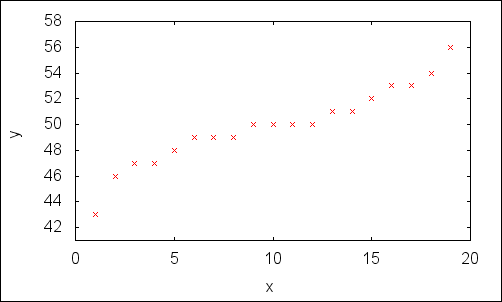
\includegraphics[width=9cm]{Siegel_Hannah_Pf14_img/Siegel_Hannah_Pf14_1.png}
\end{math}

%%%%%%%%%%%%%%%


\noindent
%%%%%%%%%%%%%%%
%%% INPUT:
\begin{minipage}[t]{8ex}{\color{red}\bf
\begin{verbatim}
(%i29) 
\end{verbatim}}
\end{minipage}
\begin{minipage}[t]{\textwidth}{\color{blue}
\begin{verbatim}
paint_TYPE1_stricherl(angabe);
\end{verbatim}}
\end{minipage}
%%% OUTPUT:
\begin{math}\displaystyle
\parbox{8ex}{\color{labelcolor}(\%t29) }
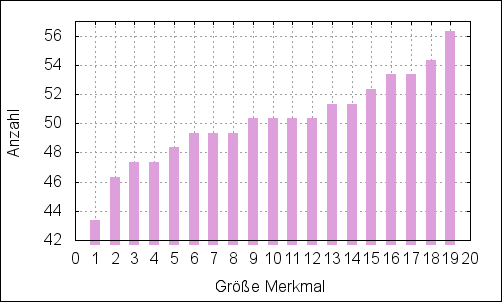
\includegraphics[width=9cm]{Siegel_Hannah_Pf14_img/Siegel_Hannah_Pf14_2.png}
\end{math}



\subsection{Absolute Haeufigkeit}


Zeichnen der absoluten Haeufigkeit fuer Kondensatoren

\noindent
%%%%%%%%%%%%%%%
%%% INPUT:
\begin{minipage}[t]{8ex}{\color{red}\bf
\begin{verbatim}
(%i30) 
\end{verbatim}}
\end{minipage}
\begin{minipage}[t]{\textwidth}{\color{blue}
\begin{verbatim}
draw_ABSOLUTE_HFG_normal(angabe,1);
\end{verbatim}}
\end{minipage}
%%% OUTPUT:
\begin{math}\displaystyle
\parbox{8ex}{\color{labelcolor}(\%t30) }
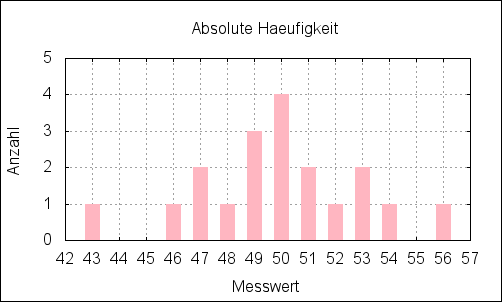
\includegraphics[width=9cm]{Siegel_Hannah_Pf14_img/Siegel_Hannah_Pf14_3.png}
\end{math}


\subsection{Relative Haeufigkeit}


Zeichnen der relativen Haeufigkeit fuer Kondensatoren

\noindent
%%%%%%%%%%%%%%%
%%% INPUT:
\begin{minipage}[t]{8ex}{\color{red}\bf
\begin{verbatim}
(%i31) 
\end{verbatim}}
\end{minipage}
\begin{minipage}[t]{\textwidth}{\color{blue}
\begin{verbatim}
draw_RELATIVE_HFG_normal(angabe,5);
\end{verbatim}}
\end{minipage}
%%% OUTPUT:
\begin{math}\displaystyle
\parbox{8ex}{\color{labelcolor}(\%t31) }
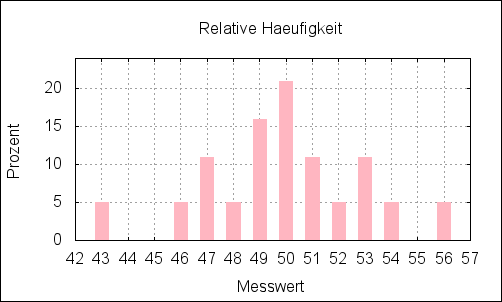
\includegraphics[width=9cm]{Siegel_Hannah_Pf14_img/Siegel_Hannah_Pf14_4.png}
\end{math}


\subsection{Kommulative absolute Haeufigkeit}


Zeichnen der Kommulativen absoluten Haeufigkeit fuer Kondensatoren

\noindent
%%%%%%%%%%%%%%%
%%% INPUT:
\begin{minipage}[t]{8ex}{\color{red}\bf
\begin{verbatim}
(%i32) 
\end{verbatim}}
\end{minipage}
\begin{minipage}[t]{\textwidth}{\color{blue}
\begin{verbatim}
draw_KUM_ABS_HFG_normal(angabe,5);
\end{verbatim}}
\end{minipage}
%%% OUTPUT:
\begin{math}\displaystyle
\parbox{8ex}{\color{labelcolor}(\%t32) }
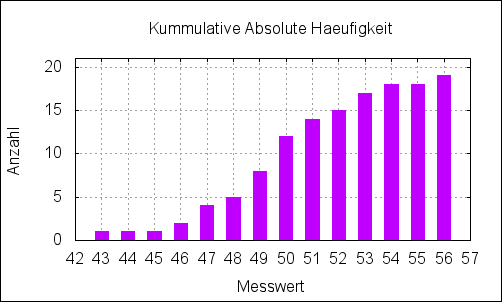
\includegraphics[width=9cm]{Siegel_Hannah_Pf14_img/Siegel_Hannah_Pf14_5.png}
\end{math}



\subsection{Kommulative relative Haeufigkeit}


Zeichnen der Kommulativen relativen Haeufigkeit fuer Kondensatoren

\noindent
%%%%%%%%%%%%%%%
%%% INPUT:
\begin{minipage}[t]{8ex}{\color{red}\bf
\begin{verbatim}
(%i33) 
\end{verbatim}}
\end{minipage}
\begin{minipage}[t]{\textwidth}{\color{blue}
\begin{verbatim}
draw_KUM_REL_HFG_normal(angabe,10);
\end{verbatim}}
\end{minipage}
%%% OUTPUT:
\begin{math}\displaystyle
\parbox{8ex}{\color{labelcolor}(\%t33) }
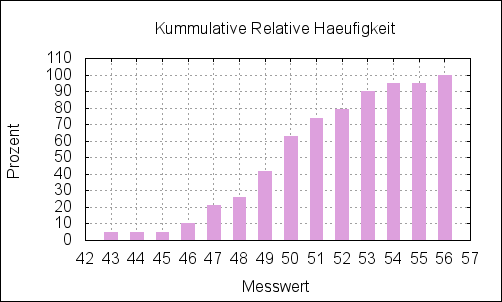
\includegraphics[width=9cm]{Siegel_Hannah_Pf14_img/Siegel_Hannah_Pf14_6.png}
\end{math}

\section{Paretto und Kreisdiagramm}



\noindent
%%%%%%%%%%%%%%%
%%% INPUT:
\begin{minipage}[t]{8ex}{\color{red}\bf
\begin{verbatim}
(%i34) 
\end{verbatim}}
\end{minipage}
\begin{minipage}[t]{\textwidth}{\color{blue}
\begin{verbatim}
kill(values);
\end{verbatim}}
\end{minipage}
%%% OUTPUT:



\subsection{Angabe }


Bei der Produktion von Blechteilen sind bei der Qualitätskontrolle folgende Fehler aufgetreten: \\
Fehler      Fehlerart   Häufigkeit \\
    1       Delle        8 \\
    2       Kratzer     26 \\
    3       Korrosion    4 \\
    4       Lackfehler  38 \\
    5       Verbogen     4 \\ 
    6       Gerissen     2 \\
    7       Maßfehler    2 \\
    8       Bohrfehler   3 \\
    9       Sonstige     3 \\

\noindent
%%%%%%%%%%%%%%%
%%% INPUT:
\begin{minipage}[t]{8ex}{\color{red}\bf
\begin{verbatim}
(%i35) 
\end{verbatim}}
\end{minipage}
\begin{minipage}[t]{\textwidth}{\color{blue}
\begin{verbatim}
urliste:[[3,Bohrfehler],[3,Sonstige],[8,Delle],[26,Kratzer],[4,Korrosion],[38,Lackfehler],[4,Verbogen],[2,Gerissen],[2,Messfehler]]$
\end{verbatim}}
\end{minipage}


\noindent
%%%%%%%%%%%%%%%
%%% INPUT:
\begin{minipage}[t]{8ex}{\color{red}\bf
\begin{verbatim}
(%i36) 
\end{verbatim}}
\end{minipage}
\begin{minipage}[t]{\textwidth}{\color{blue}
\begin{verbatim}
angabe:urliste$
\end{verbatim}}
\end{minipage}


\subsection{Pareto Diagram}



\noindent
%%%%%%%%%%%%%%%
%%% INPUT:
\begin{minipage}[t]{8ex}{\color{red}\bf
\begin{verbatim}
(%i37) 
\end{verbatim}}
\end{minipage}
\begin{minipage}[t]{\textwidth}{\color{blue}
\begin{verbatim}
draw_pareto(angabe);
\end{verbatim}}
\end{minipage}
%%% OUTPUT:
\begin{math}\displaystyle
\parbox{8ex}{\color{labelcolor}(\%t37) }
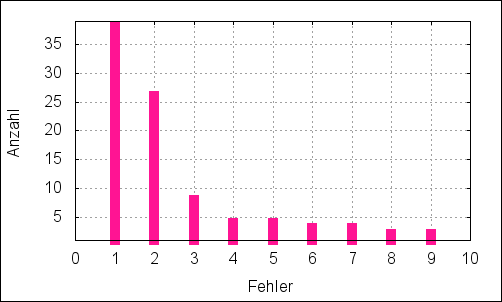
\includegraphics[width=9cm]{Siegel_Hannah_Pf14_img/Siegel_Hannah_Pf14_7.png}
\end{math}



\subsection{Kreisdiagramm}



\noindent
%%%%%%%%%%%%%%%
%%% INPUT:
\begin{minipage}[t]{8ex}{\color{red}\bf
\begin{verbatim}
(%i38) 
\end{verbatim}}
\end{minipage}
\begin{minipage}[t]{\textwidth}{\color{blue}
\begin{verbatim}
draw_piechart(angabe);
\end{verbatim}}
\end{minipage}
%%% OUTPUT:
\begin{math}\displaystyle
\parbox{8ex}{\color{labelcolor}(\%t38) }
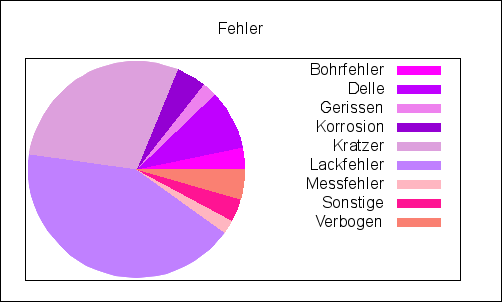
\includegraphics[width=9cm]{Siegel_Hannah_Pf14_img/Siegel_Hannah_Pf14_8.png}
\end{math}



\section{Klassenbildung}



\noindent
%%%%%%%%%%%%%%%
%%% INPUT:
\begin{minipage}[t]{8ex}{\color{red}\bf
\begin{verbatim}
(%i39) 
\end{verbatim}}
\end{minipage}
\begin{minipage}[t]{\textwidth}{\color{blue}
\begin{verbatim}
kill(values);
\end{verbatim}}
\end{minipage}



\subsection{Angabe}


Eine Messung des Füllgewichtes von 80 automatisch abgefüllten Marmeladegläsern ergab folgende Werte (in g): \\
93.0  88.2  92.1  91.0  86.9  93.8  91.0  92.0  87.4  92.1 \\
92.7  93.3  88.8  91.5  90.4  88.1  89.7  88.9  92.7  91.4 \\
89.6  89.4  87.3  86.5  90.8  90.3  86.9  91.2  89.3  90.4 \\
94.2  90.4  90.8  91.9  90.8  92.4  88.3  92.0  87.3  93.8 \\
90.6  88.0  94.0  90.9  88.0  93.1  91.7  89.7  92.7  89.5 \\
90.7  89.3  89.3  86.5  88.9  87.5  88.2  88.7  90.2  86.3 \\
93.9  86.4  90.6  87.9  85.0  89.1  91.8  92.3  87.9  95.4 

\noindent
%%%%%%%%%%%%%%%
%%% INPUT:
\begin{minipage}[t]{8ex}{\color{red}\bf
\begin{verbatim}
(%i40) 
\end{verbatim}}
\end{minipage}
\begin{minipage}[t]{\textwidth}{\color{blue}
\begin{verbatim}
messwerte:[93.9 , 86.4 , 90.6 , 87.9 , 85.0 , 89.1 , 91.8 , 92.3 , 87.9 , 95.4,90.7 , 89.3 , 89.3 , 86.5  ,88.9 , 87.5  ,88.2,  88.7,  90.2,  86.3,90.6 , 88.0 , 94.0 , 90.9 , 88.0 , 93.1,  91.7 , 89.7 , 92.7  ,89.5,94.2  ,90.4  ,90.8 , 91.9 , 90.8  ,92.4 , 88.3 , 92.0 , 87.3 , 93.8,89.6 , 89.4 , 87.3 , 86.5 , 90.8 , 90.3,  86.9,  91.2 , 89.3 , 90.4,92.7  ,93.3  ,88.8  ,91.5  ,90.4,  88.1,  89.7 , 88.9  ,92.7 , 91.4,93.0 , 88.2 , 92.1 , 91.0,  86.9,  93.8 , 91.0  ,92.0,  87.4 , 92.1]$
\end{verbatim}}
\end{minipage}


\subsection{Theorie}


Es herrscht bei dieser Angabe folgendes Problem: 80 Balken und alle sind ca geich gross aber doch nicht genau gleich (unterschied nach dem Komma). \\
Daher: teilen in Klassen (e.g. unter 85, zwische 85 und 90, zwischen 90 und 95 ... ueber 110)
\\ \\
Bei der Klassenbildung gilt immer dass: \\
    durch einen VERLUST an INFORMATION gleichzeitig ein GEWINN an UEBERSICHTLICHKEIT der Darstellung
\\ \\
SCHRITTE ZUR KLASSENBILDUNG \\
    (1) Die Klassengrenzen sollen moeglichst einfache Zahlen sein, welche genau sind allerdings von den Eingangsdaten abhaengig \\
    (2) Unterste und oberste Klasse werden so gewaehlt, dass der kleinstwert und der groesstwert drinnenliegt. \\
    (3) Wenn m die STICHPROBEN: meistens sqrt(m) aber immer \verb|<|= 20 Klassen \\
    (4) Die Klassenbreiten sollten gleich gross gewaehlt werden (mit ausnahme der 1. und letzten Klasse) \\
    (5) Klassen breite W:   wenn n \verb|<|= 400 --\verb|>| W = (xmax - xmin) / sqrt(n) --\verb|>| Ergebniss runden
                            wenn n \verb|>| 400 --\verb|>| W = (xmax - xmin) / 20 --\verb|>| Ergebniss runden
\\ \\
Die Urliste wird durch die Klasseneinteilung (welche dokumentiert und begruendet werden muss) in eine neue liste eingetragen \\
Diese Liste hat das Format: [1,2,6,2,8,3,5,1,5,7,8,3,7,... ] und kann somit wieder interpretiert werden.

\subsection{Klassenbildung}


(2) \\
Kleinstwert(xmin) und Groesstwert (xmax)

\noindent
%%%%%%%%%%%%%%%
%%% INPUT:
\begin{minipage}[t]{8ex}{\color{red}\bf
\begin{verbatim}
(%i41) 
\end{verbatim}}
\end{minipage}
\begin{minipage}[t]{\textwidth}{\color{blue}
\begin{verbatim}
kleinstwert: lmin(messwerte);
groesstwert: lmax(messwerte);
\end{verbatim}}
\end{minipage}
%%% OUTPUT:
\begin{math}\displaystyle
\parbox{8ex}{\color{labelcolor}(\%o41) }
85.0
\end{math}

\begin{math}\displaystyle
\parbox{8ex}{\color{labelcolor}(\%o42) }
95.40000000000001
\end{math}
%%%%%%%%%%%%%%%

(3) \\
Anzahl der Messwerte

\noindent
%%%%%%%%%%%%%%%
%%% INPUT:
\begin{minipage}[t]{8ex}{\color{red}\bf
\begin{verbatim}
(%i43) 
\end{verbatim}}
\end{minipage}
\begin{minipage}[t]{\textwidth}{\color{blue}
\begin{verbatim}
anzahl_messwerte:length(messwerte);
\end{verbatim}}
\end{minipage}
%%% OUTPUT:


(3) \\
Anzahl der Klassen

\noindent
%%%%%%%%%%%%%%%
%%% INPUT:
\begin{minipage}[t]{8ex}{\color{red}\bf
\begin{verbatim}
(%i44) 
\end{verbatim}}
\end{minipage}
\begin{minipage}[t]{\textwidth}{\color{blue}
\begin{verbatim}
anzahl_klassen:(sqrt(anzahl_messwerte)),numer;
\end{verbatim}}
\end{minipage}
%%% OUTPUT:
\begin{math}\displaystyle
\parbox{8ex}{\color{labelcolor}(\%o44) }
8.366600265340756
\end{math}
%%%%%%%%%%%%%%%


\noindent
%%%%%%%%%%%%%%%
%%% INPUT:
\begin{minipage}[t]{8ex}{\color{red}\bf
\begin{verbatim}
(%i45) 
\end{verbatim}}
\end{minipage}
\begin{minipage}[t]{\textwidth}{\color{blue}
\begin{verbatim}
anzahl_klassen:round(anzahl_klassen);
\end{verbatim}}
\end{minipage}
%%% OUTPUT:
\begin{math}\displaystyle
\parbox{8ex}{\color{labelcolor}(\%o45) }
8
\end{math}
%%%%%%%%%%%%%%%

(4)
Klassenbreite

\noindent
%%%%%%%%%%%%%%%
%%% INPUT:
\begin{minipage}[t]{8ex}{\color{red}\bf
\begin{verbatim}
(%i46) 
\end{verbatim}}
\end{minipage}
\begin{minipage}[t]{\textwidth}{\color{blue}
\begin{verbatim}
W = ((groesstwert - kleinstwert) / anzahl_klassen),numer;
\end{verbatim}}
\end{minipage}
%%% OUTPUT:
\begin{math}\displaystyle
\parbox{8ex}{\color{labelcolor}(\%o46) }
W=1.300000000000001
\end{math}
%%%%%%%%%%%%%%%

KLASSENBILDUNG \\
Das Ergebniss aus (3) und (4) muss nun interpretiert werden. \\
Da nur ganzzahlige Klassen gebildet werden koennen, sollten entweder 8 oder 9 Klassen gebildet werden.\\
Die Klassenbreite soll bei etwa 1.3 liegen. Da dies eine nicht sehr schoene Zahl ist, kann man entwender 1.25 oder 1.5 waehlen. \\
Wir waehlen nun folgende werte: \\
1.25 und 8

\noindent
%%%%%%%%%%%%%%%
%%% INPUT:
\begin{minipage}[t]{8ex}{\color{red}\bf
\begin{verbatim}
(%i47) 
\end{verbatim}}
\end{minipage}
\begin{minipage}[t]{\textwidth}{\color{blue}
\begin{verbatim}
steps:1.25;
anzahl_klassen:8;
\end{verbatim}}
\end{minipage}
%%% OUTPUT:
\begin{math}\displaystyle
\parbox{8ex}{\color{labelcolor}(\%o47) }
1.25
\end{math}

\begin{math}\displaystyle
\parbox{8ex}{\color{labelcolor}(\%o48) }
8
\end{math}
%%%%%%%%%%%%%%%

Aufruf des Blockes \\
Return value anzusprechen: end\_wert (klasseneingeteilt) , klassen (die eingeteilt wurden)

\noindent
%%%%%%%%%%%%%%%
%%% INPUT:
\begin{minipage}[t]{8ex}{\color{red}\bf
\begin{verbatim}
(%i49) 
\end{verbatim}}
\end{minipage}
\begin{minipage}[t]{\textwidth}{\color{blue}
\begin{verbatim}
klassenbildung(messwerte,steps,anzahl_klassen);
\end{verbatim}}
\end{minipage}
%%% OUTPUT:
\begin{math}\displaystyle
\parbox{8ex}{\color{labelcolor}(\%o49) }
done
\end{math}
%%%%%%%%%%%%%%%

'Probe':

\noindent
%%%%%%%%%%%%%%%
%%% INPUT:
\begin{minipage}[t]{8ex}{\color{red}\bf
\begin{verbatim}
(%i50) 
\end{verbatim}}
\end{minipage}
\begin{minipage}[t]{\textwidth}{\color{blue}
\begin{verbatim}
length(end_list)=length(messwerte);
\end{verbatim}}
\end{minipage}
%%% OUTPUT:
\begin{math}\displaystyle
\parbox{8ex}{\color{labelcolor}(\%o50) }
70=70
\end{math}
%%%%%%%%%%%%%%%


\subsection{Grafische Darstellung der Klassen}


Sollten die Werte (Labels) sich ueberschneiden, weil zu viele klassen geawehlt sind, muss man jediglich:
- den letzten sowie den vorletzten Wert variieren, bis die Grafik schoen ist. \\
Die Default values koennen mit 0 angesprochen werden, oder einfach eingegeben werden ([500,300])
\\ \\
Die schon oben angefuehrte Erklaerung der draw Bloecke: \\
    Jeder draw\_TYPE\_klassen Block, macht die Klasseneinteilung sowie das Zeichnen mit den Labels automatisch. \\ \\

draw\_TYPE\_klassen(messwerte,steps,anzahl\_klasse,ytics,minus\_delta,xdimension,ydimension)
\\ \\
messwerte ... Eine Liste der messwerte im Format [Messwert1, Messwert2, ...] \\
steps ... Die Klassenbreite W \\
anzahl\_klassen ... Anzahl der Klassen \\
ytics ... Abstand der Werte auf der y-Achse (Default:5) \\
minus\_delta ... POSITIVER Wert, range fuer das anzeigen der Labels (sollte meist zwischen ca 5 und 20 liegen) (Default:10) \\
xdimension ... Groesse der Zeichnung nach x (Default:500) \\
ydimension ... Groesse der Zeichnung nach y (Default:300) \\

Zeichnen der absoluten Haeufigkeit

\noindent
%%%%%%%%%%%%%%%
%%% INPUT:
\begin{minipage}[t]{8ex}{\color{red}\bf
\begin{verbatim}
(%i51) 
\end{verbatim}}
\end{minipage}
\begin{minipage}[t]{\textwidth}{\color{blue}
\begin{verbatim}
draw_ABSOLUTE_HFG_klassen(messwerte,steps,anzahl_klassen,0,0,0,0);
\end{verbatim}}
\end{minipage}
%%% OUTPUT:
\begin{math}\displaystyle
\parbox{8ex}{\color{labelcolor}(\%t51) }
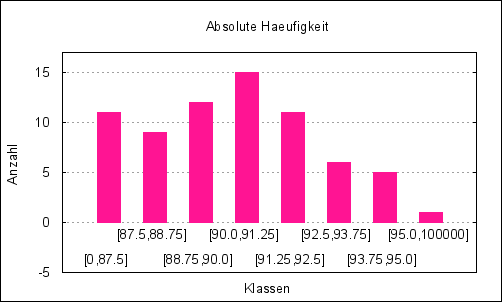
\includegraphics[width=9cm]{Siegel_Hannah_Pf14_img/Siegel_Hannah_Pf14_9.png}
\end{math}

%%%%%%%%%%%%%%%

Zeichnen der relativen Haeufigkeit

\noindent
%%%%%%%%%%%%%%%
%%% INPUT:
\begin{minipage}[t]{8ex}{\color{red}\bf
\begin{verbatim}
(%i52) 
\end{verbatim}}
\end{minipage}
\begin{minipage}[t]{\textwidth}{\color{blue}
\begin{verbatim}
draw_RELATIVE_HFG_klassen(messwerte,steps,anzahl_klassen,0,0,0,0);
\end{verbatim}}
\end{minipage}
%%% OUTPUT:
\begin{math}\displaystyle
\parbox{8ex}{\color{labelcolor}(\%t52) }
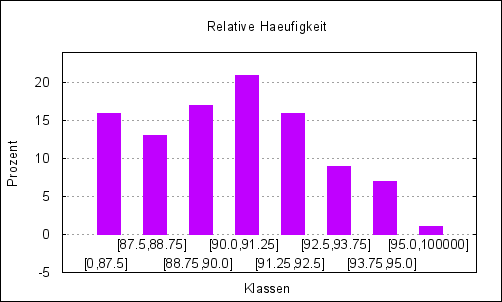
\includegraphics[width=9cm]{Siegel_Hannah_Pf14_img/Siegel_Hannah_Pf14_10.png}
\end{math}

%%%%%%%%%%%%%%%

Zeichnen der Kommulativen absoluten Haeufigkeit

\noindent
%%%%%%%%%%%%%%%
%%% INPUT:
\begin{minipage}[t]{8ex}{\color{red}\bf
\begin{verbatim}
(%i53) 
\end{verbatim}}
\end{minipage}
\begin{minipage}[t]{\textwidth}{\color{blue}
\begin{verbatim}
draw_KUM_ABS_HFG_klassen(messwerte,steps,anzahl_klassen,10,20,0,0);
\end{verbatim}}
\end{minipage}
%%% OUTPUT:
\begin{math}\displaystyle
\parbox{8ex}{\color{labelcolor}(\%t53) }
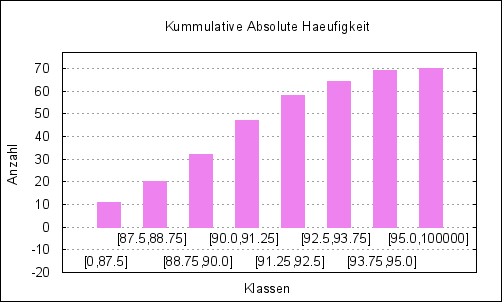
\includegraphics[width=9cm]{Siegel_Hannah_Pf14_img/Siegel_Hannah_Pf14_11.png}
\end{math}



\subsection{Kommulative relative Haeufigkeit}


Zeichnen der Kommulativen relativen Haeufigkeit

\noindent
%%%%%%%%%%%%%%%
%%% INPUT:
\begin{minipage}[t]{8ex}{\color{red}\bf
\begin{verbatim}
(%i54) 
\end{verbatim}}
\end{minipage}
\begin{minipage}[t]{\textwidth}{\color{blue}
\begin{verbatim}
draw_KUM_REL_HFG_klassen(messwerte,steps,anzahl_klassen,10,20,0,0);
\end{verbatim}}
\end{minipage}
%%% OUTPUT:
\begin{math}\displaystyle
\parbox{8ex}{\color{labelcolor}(\%t54) }
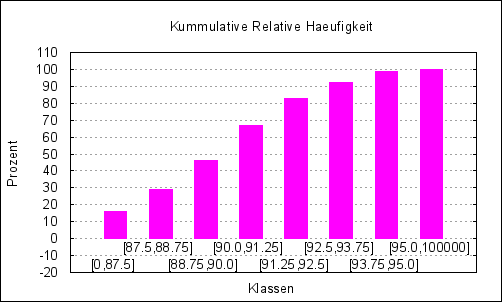
\includegraphics[width=9cm]{Siegel_Hannah_Pf14_img/Siegel_Hannah_Pf14_12.png}
\end{math}



\section{Kenngroessen}



\noindent
%%%%%%%%%%%%%%%
%%% INPUT:
\begin{minipage}[t]{8ex}{\color{red}\bf
\begin{verbatim}
(%i55) 
\end{verbatim}}
\end{minipage}
\begin{minipage}[t]{\textwidth}{\color{blue}
\begin{verbatim}
kill (allbut (rand_col));
load(descriptive)$
load(draw)$
\end{verbatim}}
\end{minipage}



\subsection{Angabe}


Aus einer Lieferung von elektrischen Widerständen gleicher Art werden einige Stück herausgegriffen und gemessen.  \\
Dabei werden folgende Werte (in Ohm) gefunden:

\noindent
%%%%%%%%%%%%%%%
%%% INPUT:
\begin{minipage}[t]{8ex}{\color{red}\bf
\begin{verbatim}
(%i3) 
\end{verbatim}}
\end{minipage}
\begin{minipage}[t]{\textwidth}{\color{blue}
\begin{verbatim}
urliste:[98.7,  99.3,  95.8,  101.6,  100.4 , 98.0 , 96.3];
\end{verbatim}}
\end{minipage}
%%% OUTPUT:
\begin{math}\displaystyle
\parbox{8ex}{\color{labelcolor}(\%o3) }
[98.7,99.3,95.8,101.6,100.4,98.0,96.3]
\end{math}
%%%%%%%%%%%%%%%


\noindent
%%%%%%%%%%%%%%%
%%% INPUT:
\begin{minipage}[t]{8ex}{\color{red}\bf
\begin{verbatim}
(%i4) 
\end{verbatim}}
\end{minipage}
\begin{minipage}[t]{\textwidth}{\color{blue}
\begin{verbatim}
angabe:urliste$
\end{verbatim}}
\end{minipage}


\subsection{Minima und Maxima}


minimalwert

\noindent
%%%%%%%%%%%%%%%
%%% INPUT:
\begin{minipage}[t]{8ex}{\color{red}\bf
\begin{verbatim}
(%i5) 
\end{verbatim}}
\end{minipage}
\begin{minipage}[t]{\textwidth}{\color{blue}
\begin{verbatim}
smin(angabe);
\end{verbatim}}
\end{minipage}
%%% OUTPUT:
\begin{math}\displaystyle
\parbox{8ex}{\color{labelcolor}(\%o5) }
95.8
\end{math}
%%%%%%%%%%%%%%%

maximalwert

\noindent
%%%%%%%%%%%%%%%
%%% INPUT:
\begin{minipage}[t]{8ex}{\color{red}\bf
\begin{verbatim}
(%i6) 
\end{verbatim}}
\end{minipage}
\begin{minipage}[t]{\textwidth}{\color{blue}
\begin{verbatim}
smax(angabe);
\end{verbatim}}
\end{minipage}
%%% OUTPUT:
\begin{math}\displaystyle
\parbox{8ex}{\color{labelcolor}(\%o6) }
101.6
\end{math}
%%%%%%%%%%%%%%%


\subsection{Mittelwert}


Arithmetischer Mittelwert

\noindent
%%%%%%%%%%%%%%%
%%% INPUT:
\begin{minipage}[t]{8ex}{\color{red}\bf
\begin{verbatim}
(%i7) 
\end{verbatim}}
\end{minipage}
\begin{minipage}[t]{\textwidth}{\color{blue}
\begin{verbatim}
mean(angabe);
\end{verbatim}}
\end{minipage}
%%% OUTPUT:
\begin{math}\displaystyle
\parbox{8ex}{\color{labelcolor}(\%o7) }
98.58571428571428
\end{math}
%%%%%%%%%%%%%%%

Geometrischer Mittelwert

\noindent
%%%%%%%%%%%%%%%
%%% INPUT:
\begin{minipage}[t]{8ex}{\color{red}\bf
\begin{verbatim}
(%i8) 
\end{verbatim}}
\end{minipage}
\begin{minipage}[t]{\textwidth}{\color{blue}
\begin{verbatim}
geometric_mean (angabe);
\end{verbatim}}
\end{minipage}
%%% OUTPUT:
\begin{math}\displaystyle
\parbox{8ex}{\color{labelcolor}(\%o8) }
98.56670574148326
\end{math}
%%%%%%%%%%%%%%%

Harmonischer Mittelwert

\noindent
%%%%%%%%%%%%%%%
%%% INPUT:
\begin{minipage}[t]{8ex}{\color{red}\bf
\begin{verbatim}
(%i9) 
\end{verbatim}}
\end{minipage}
\begin{minipage}[t]{\textwidth}{\color{blue}
\begin{verbatim}
harmonic_mean(angabe);
\end{verbatim}}
\end{minipage}
%%% OUTPUT:
\begin{math}\displaystyle
\parbox{8ex}{\color{labelcolor}(\%o9) }
98.54769453535242
\end{math}
%%%%%%%%%%%%%%%


\subsection{Median}



\noindent
%%%%%%%%%%%%%%%
%%% INPUT:
\begin{minipage}[t]{8ex}{\color{red}\bf
\begin{verbatim}
(%i10) 
\end{verbatim}}
\end{minipage}
\begin{minipage}[t]{\textwidth}{\color{blue}
\begin{verbatim}
median(angabe);
\end{verbatim}}
\end{minipage}
%%% OUTPUT:
\begin{math}\displaystyle
\parbox{8ex}{\color{labelcolor}(\%o10) }
98.7
\end{math}
%%%%%%%%%%%%%%%

Ein Median und ein Mittelwert entsprechen sich dann, wenn man keine Werte hat, bei welchen die Randwerte extrem sind.

\subsection{Standardabweichung}



\noindent
%%%%%%%%%%%%%%%
%%% INPUT:
\begin{minipage}[t]{8ex}{\color{red}\bf
\begin{verbatim}
(%i11) 
\end{verbatim}}
\end{minipage}
\begin{minipage}[t]{\textwidth}{\color{blue}
\begin{verbatim}
std(angabe);
\end{verbatim}}
\end{minipage}
%%% OUTPUT:
\begin{math}\displaystyle
\parbox{8ex}{\color{labelcolor}(\%o11) }
1.935701106966209
\end{math}
%%%%%%%%%%%%%%%


\subsection{Varianz}


Varianz dividiert durch n

\noindent
%%%%%%%%%%%%%%%
%%% INPUT:
\begin{minipage}[t]{8ex}{\color{red}\bf
\begin{verbatim}
(%i12) 
\end{verbatim}}
\end{minipage}
\begin{minipage}[t]{\textwidth}{\color{blue}
\begin{verbatim}
var(angabe);
\end{verbatim}}
\end{minipage}
%%% OUTPUT:
\begin{math}\displaystyle
\parbox{8ex}{\color{labelcolor}(\%o12) }
3.746938775510206
\end{math}
%%%%%%%%%%%%%%%

Varianz dividiert durch n-1 (= Fuer groesse Mengen an daten)

\noindent
%%%%%%%%%%%%%%%
%%% INPUT:
\begin{minipage}[t]{8ex}{\color{red}\bf
\begin{verbatim}
(%i13) 
\end{verbatim}}
\end{minipage}
\begin{minipage}[t]{\textwidth}{\color{blue}
\begin{verbatim}
var1(angabe);
\end{verbatim}}
\end{minipage}
%%% OUTPUT:
\begin{math}\displaystyle
\parbox{8ex}{\color{labelcolor}(\%o13) }
4.371428571428574
\end{math}
%%%%%%%%%%%%%%%


\subsection{Spannweite}



\noindent
%%%%%%%%%%%%%%%
%%% INPUT:
\begin{minipage}[t]{8ex}{\color{red}\bf
\begin{verbatim}
(%i14) 
\end{verbatim}}
\end{minipage}
\begin{minipage}[t]{\textwidth}{\color{blue}
\begin{verbatim}
range(angabe);
\end{verbatim}}
\end{minipage}
%%% OUTPUT:
\begin{math}\displaystyle
\parbox{8ex}{\color{labelcolor}(\%o14) }
5.799999999999997
\end{math}
%%%%%%%%%%%%%%%


\subsection{Quartile}


unteres Quartil

\noindent
%%%%%%%%%%%%%%%
%%% INPUT:
\begin{minipage}[t]{8ex}{\color{red}\bf
\begin{verbatim}
(%i15) 
\end{verbatim}}
\end{minipage}
\begin{minipage}[t]{\textwidth}{\color{blue}
\begin{verbatim}
quantile (angabe, 0.25);
\end{verbatim}}
\end{minipage}
%%% OUTPUT:
\begin{math}\displaystyle
\parbox{8ex}{\color{labelcolor}(\%o15) }
97.15000000000001
\end{math}
%%%%%%%%%%%%%%%

oberes Quartil

\noindent
%%%%%%%%%%%%%%%
%%% INPUT:
\begin{minipage}[t]{8ex}{\color{red}\bf
\begin{verbatim}
(%i16) 
\end{verbatim}}
\end{minipage}
\begin{minipage}[t]{\textwidth}{\color{blue}
\begin{verbatim}
quantile (angabe, 0.75);
\end{verbatim}}
\end{minipage}
%%% OUTPUT:
\begin{math}\displaystyle
\parbox{8ex}{\color{labelcolor}(\%o16) }
99.84999999999999
\end{math}
%%%%%%%%%%%%%%%


\subsection{Grafische Darstellung mittels Boxplot}



\noindent
%%%%%%%%%%%%%%%
%%% INPUT:
\begin{minipage}[t]{8ex}{\color{red}\bf
\begin{verbatim}
(%i17) 
\end{verbatim}}
\end{minipage}
\begin{minipage}[t]{\textwidth}{\color{blue}
\begin{verbatim}
wxboxplot(angabe,box_orientation=horizontal,box_width=0.25,color=rand_col(1),line_width=2, title="Lieferung von elektrischen Widerständen ");
\end{verbatim}}
\end{minipage}
%%% OUTPUT:
\begin{math}\displaystyle
\parbox{8ex}{\color{labelcolor}(\%t17) }
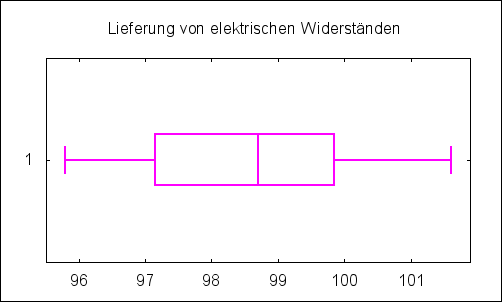
\includegraphics[width=9cm]{Siegel_Hannah_Pf14_img/Siegel_Hannah_Pf14_13.png}
\end{math}



\end{document}
